\documentclass[a4paper]{article}
\usepackage{graphicx,subcaption}
\usepackage{amsmath,amsfonts}
\title{Fundamentals of Financial Forecasting}
\author{G.A. Jarrad}
\begin{document}
\maketitle
\numberwithin{equation}{section}
\numberwithin{figure}{section}
\numberwithin{table}{section}
\section{Introduction}\label{sec:intro}
A typical goal in the financial arena is to attempt to predict the future based upon knowledge of the past, in order to make profitable trades.
In this document, we shall look primarily at the analysis of financial timeseries data, in particular the prices of stocks.
For illustrative purposes, most of our examples will be drawn from the analysis of the price history of just a few stocks, as shown
in Figure~\ref{fig:stock-prices}. Of course, in practice one must collect and analyse a large amount of data for a wide variety of stocks, 
in order to obtain more general and robust predictive models.

\section{Basic Time-Series Modelling}

\subsection{Predictive Model}
Consider the stock prices shown in Figure~\ref{fig:stock-prices},
which vary daily over a period of time.
Each sequence of prices for a given stock forms a time-series.
Here let $V(t)$ be the price of a given stock at time $t$. In general,
$V(t)$ represents the time-varying value of any asset. We
consider only the gross, not net, asset value, and hence may assume that $V(t)\ge 0$.
\begin{figure}[hbt]
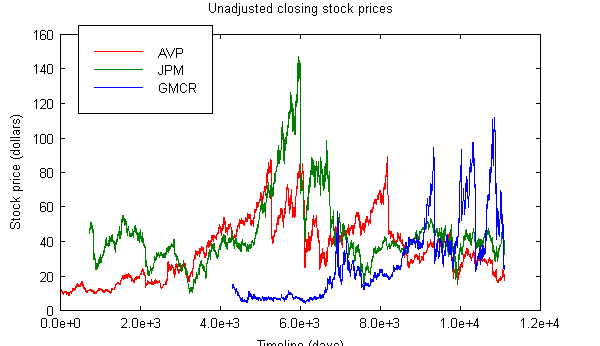
\includegraphics[scale=0.8]{figures/stock-prices-close.png}
\caption{Example data showing the unadjusted closing prices of three different
types of stock.}
\label{fig:stock-prices}
\end{figure}

Now, suppose for the purpose of illustration that
we buy an asset, e.g. a parcel of shares in a stock, at time $t$ for amount $V(t)$ and then sell it at a later
time $t+T$ for value $V(t+T)$. Then the difference in asset values is the
{\em profit}, or {\em return}, on our investment, namely
\begin{eqnarray}
  P(t,t+T) & = & V(t+T)-V(t)\,,
\end{eqnarray}
as shown in Figure~\ref{fig:avp-price-diff}.
Of key importance, therefore, is to attempt to define a predictive model
that estimates the future value $V(t+T)$ given the current value $V(t)$.
\begin{figure}[hbt]
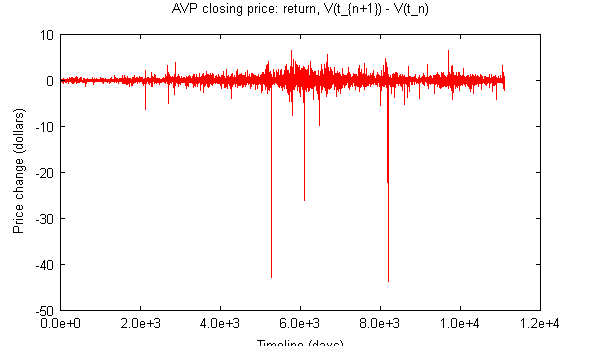
\includegraphics[scale=0.8]{figures/avp-price-close-diff.png}
\caption{Example time-series of the daily return in closing price
of AVP stock.}
\label{fig:avp-price-diff}
\end{figure}

Now, observe that the return has the same currency units as
the asset value. Thus, as an alternative, we might instead 
consider the profit per unit of investment, which is
a dimensionless measure 
known as the {\em relative return}, given by
\begin{eqnarray}
  Q(t,t+T) & = & \frac{V(t+T)-V(t)}{V(t)}\,.
\end{eqnarray}
An example of the relative return 
is shown in Figure~\ref{fig:avp-price-simple}.
Of more use, however,  is
the relative return on the investment per unit time, given by
\begin{eqnarray}
  R(t,t+T) & = & \frac{V(t+T)-V(t)}{T\;V(t)}\,.
\end{eqnarray}
This is known as the {\em rate of return}, and
is show in Figure~\ref{fig:avp-price-log}.
\begin{figure}[hbt]
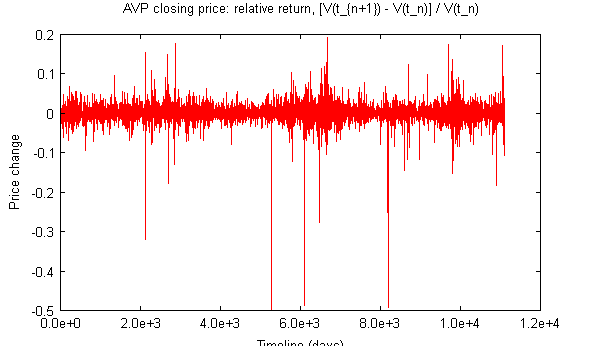
\includegraphics[scale=0.8]{figures/avp-price-close-simple.png}
\caption{Example time-series of the daily relative return of
the closing price of AVP stock.}
\label{fig:avp-price-simple}
\end{figure}
\begin{figure}[hbt]
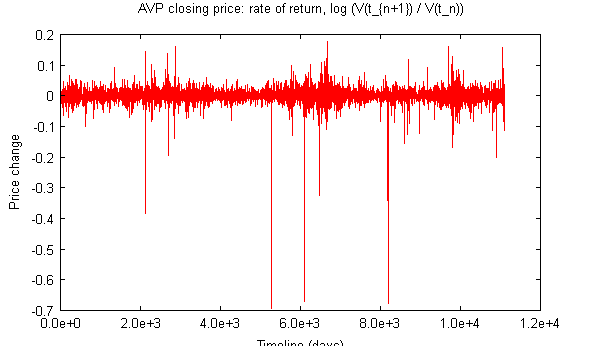
\includegraphics[scale=0.8]{figures/avp-price-close-log.png}
\caption{Example time-series of the daily rate of return of
the closing price of AVP stock.}
\label{fig:avp-price-log}
\end{figure}

Next, observe that as the length $T$ of the predictive interval 
$[t,t+T]$ becomes vanishingly small, we obtain the 
{\em instantaneous rate of return}
given by
\begin{eqnarray}
  r(t) & = & \lim_{T\rightarrow 0}\frac{V(t+T)-V(t)}{T\;V(t)}
 ~=~\frac{V'(t)}{V(t)}\,.
\label{eq:inst-rate-return}
\end{eqnarray}
In order to relate $r(t)$ to a predictive model of $V(t+T)$,
note from the derivative chain rule that 
\begin{eqnarray}
  \frac{d\;\ln V(t)}{dt} & = & \frac{V'(t)}{V(t)}~=~r(t)\,.
\end{eqnarray}
Hence, by integrating this instantaneous rate of return
over the interval $[t,t+T]$ we obtain
\begin{eqnarray}
  \ln V(t+T) & = & \ln V(t) + T\;\bar{R}(t,t+T)\,,
\label{eq:log-V-bar-R}
\end{eqnarray}
where $\bar{R}(t,t+T)$ is the {\em average} rate of return 
over the interval, given by
\begin{eqnarray}
  \bar{R}(t,t+T) & = & \frac{1}{T}\int_{t}^{t+T}r(t)\;dt\,.
\label{eq:bar-R-def}
\end{eqnarray}
Note that $\bar{R}(t,t+T)$ has 
the useful property of
having the unrestricted range $(-\infty,\infty)$, 
despite the fact that $V(t)$ has the restricted range $[0,\infty)$.

Finally, observe for the sake of completeness that
equation~(\ref{eq:log-V-bar-R}) can be rearranged to give
\begin{eqnarray}
  \bar{R}(t,t+T) & = &  \frac{1}{T}\ln\frac{V(t+T)}{V(t)}\,,
\end{eqnarray}
which is thus also known as the {\em logarithmic} rate of return.
Likewise, equation~(\ref{eq:log-V-bar-R}) can be rearranged to give
\begin{eqnarray}
  V(t+T) & = & V(t)\;e^{T\;\bar{R}(t,t+T)}\,,
\end{eqnarray}
such that $\bar{R}(t,t+T)$ 
is also known
as the {\em continuously compounded} rate of return, due to the fact that
\begin{eqnarray}
e^{T\;\bar{R}(t,t+T)} & = & 
\lim_{N\rightarrow\infty}\left(1+\frac{T\;\bar{R}(t,t+T)}{N}\right)^{N}\,.
\end{eqnarray}

\subsection{Stochastic Model}

In practice, the average rate of return
is often treated synonymously with the instantaneous
rate of return. This is because, 
from the Mean Value Theorem 
(for example, see equation~(\ref{eq:mean-value-theorem}) from Appendix~\ref{sec:mean-value-theorem}),
there is a value $\xi\in[t,t+T]$ such that $\bar{R}(t,t+T)=r(\xi)$.
In other words, the averate rate of return over an interval equals the instantaneous rate of return at some point in the interval.

Since the value of $\xi$ is unknown, we may treat it as a random variable,
and by extension $\bar{R}(t,t+T)$ is also a random variable.
It remains to decide how to model
its stochastic distribution.
In order to do this, first reconsider
the stock prices shown in Figure~\ref{fig:stock-prices}.
Although the value $V(t)$ of an asset is assumed to vary continuously with time $t$, the example stock prices were in
fact sampled at the close of each day of trading.
Thus, in general, rather than knowing $V(t)$ for all $t$, we only know
values $V(t_i)$ sampled at discrete times $t_i$,
for $i=0,1,\ldots,N$. The length of time $\delta t_i=t_i-t_{i-1}$ 
between samples is sometimes known as a {\em bar}.
For the example stock prices, each bar is fixed equal to 1 day.

In terms of the prediction interval $[t,t+T]$, let us now arbitrarily
define $t_0=t$ and $t_n=t+T$ for some integer $n>0$.
Then $[t,t+T]$ may be partitioned into $n$ subintervals $[t_{i-1},t_i]$
for $i=1,2,\ldots,n$. Then, from definition~(\ref{eq:bar-R-def}),
we obtain
\begin{eqnarray}
(t_n-t_0)\bar{R}(t_0,t_n) & = & 
(t_1-t_0)\bar{R}(t_0,t_1)+\cdots
+(t_n-t_{n-1})\bar{R}(t_{n-1},t_n)\nonumber\\
& = & 
\sum_{i=1}^n \delta t_i\;\bar{R}(t_{i-1},t_i)\,,
\label{eq:R-bar-partition}
\end{eqnarray}
where $\bar{R}(t_{i-1},t_i)$ is just the average rate of return
over the subinterval $[t_{i-1},t_i]$. Hence,
we treat each $\bar{R}(t_{i-1},t_i)$ as a random variable
in its own right. 

Turning briefly to sampling theory, note that if a random variable X
is distributed with mean $\mu$ and variance $\sigma^2$, then
the mean $\bar{X}$ of $n$ random samples, each indpendently and
identically drawn from the same distribution for $X$, 
is itself distributed with mean $\mu$
and variance $\sigma^2/n$.
We therefore invoke several key assumptions:
\begin{enumerate}
\item {\em Independence}: 
Each variable $\bar{R}(t_{i-1},t_{i})$ is independently distributed
from any other variable $\bar{R}(t_{j-1},t_{j})$ for $j\ne i$.

\item {\em Memorylessness}: The distribution of
$\bar{R}(t_i,t_{i-1})$ depends only 
upon the length
$\delta t_i=t_i-t_{i-1}$ of the subinterval $[t_{i-1},t_i]$ and not
upon its endpoints.

\item {\em Identity}: Any two distinct variables 
$\bar{R}(t_i,t_{i-1})$ and $\bar{R}(t_{j-1},t_{j})$, for $j\ne i$,
are identically distributed if $\delta t_i=\delta t_j$. 
\end{enumerate}
As a consequence of the assumptions of memorylessness and identity, 
we may suppose that
\begin{eqnarray}
\mbox{E}[\bar{R}(t_i,t_{i-1})]~=~m(\delta t_i)\;\mu, &&
\mbox{Var}[\bar{R}(t_i,t_{i-1})]~=~v(\delta t_i)\;\sigma^2\,,
\end{eqnarray}
for unknown functions $m(\delta t)$ and $v(\delta t)$.
Thus, taking the expectation of equation~(\ref{eq:R-bar-partition}) gives
\begin{eqnarray}
(t_n-t_0)\;m(t_n-t_0)\;\mu & = & 
\sum_{i=1}^{n}\delta t_i\;m(\delta t_i)\;\mu\,,
\end{eqnarray}
which is satisfied by choosing $m(\delta t)=1$.
Similarly, making use of the independence assmuption, taking the variance of eqaution~(\ref{eq:R-bar-partition})
gives
\begin{eqnarray}
(t_n-t_0)^2 \;v(t_n-t_0)\;\sigma^2 & = & 
\sum_{i=1}^{n}(\delta t_i)^2\;v(\delta t_i)\;\sigma^2\,,
\end{eqnarray}
which is satisfied by choosing $v(\delta t)=1/\delta t$. 
Therefore, we conclude that, over the arbitrary interval $[t,t+T]$, the continuous analogue to the discrete sample mean is given by
\begin{eqnarray}
\mbox{E}[\bar{R}(t,t+T)]~=~\mu, &&
\mbox{Var}[\bar{R}(t,t+T)]~=~\frac{\sigma^2}{T}\,.
\end{eqnarray}

\subsection{Relative Returns}
Suppose, for the sake of argument, that we invest an initial amount
$V(t_0)$ in a bank that offers an annual rate of interest compunded
$n$ times a year. Then, letting $S_i$ be the relative return
over the interval $t\in[t_0+(i-1)\delta t,t_0+i\delta t]$, the
value of our investment after one year is given by
\begin{eqnarray}
V(t_0+n\delta t) & = & V(t_0)\prod_{i=1}^{n}(1+S_i)\,.
\label{eq:Vn-compound}
\end{eqnarray}
Next, suppose that the interest rate is fixed, such that each 
$S_i$ is constant. Then equation~(\ref{eq:Vn-compound}) becomes
\begin{eqnarray}
V(t_0+n\delta t) & = & V(t_0)(1+\bar{S})^{n}
\,\,\,\mbox{for $S_i$ constant}\,,
\label{eq:Vn:Sbar}
\end{eqnarray}
where $\bar{S}$ is the arithmentic mean of
$n$ values of some generic relative return $S$, defined by
\begin{eqnarray}
1+\bar{S} & = & A_n(1+S)~=~\frac{1}{n}\sum_{i=1}^{n}(1+S_i)\,.
\end{eqnarray}
In contrast, suppose instead that the interest rate is now variable, 
such that $S_i$ is no longer constant.
Then equation~(\ref{eq:Vn-compound}) becomes
\begin{eqnarray}
V(t_0+n\delta t) & = & V(t_0)(1+\tilde{S})^{n}
\,\,\,\mbox{for $S_i$ variable}\,,
\label{eq:Vn:Stilde}
\end{eqnarray}
where $\tilde{S}$ is the geometrically-adjusted mean relative return,
defined by
\begin{eqnarray}
1+\tilde{S} & = & G_n(1+S)~=~
\left[\prod_{i=1}^{n}(1+S_i)\right]^{\frac{1}{n}}\,.
\label{eq:Gn:def}
\end{eqnarray}
Now, it is known that for any variable $X$, we have $G_n(X)\le A_n(X)$, where the
equality occurs only when the values of $X$ are constant.
Hence, from equations~(\ref{eq:Vn:Sbar}) and (\ref{eq:Vn:Stilde}),
we observe that
\begin{eqnarray}
V(t_0+n\delta t) & = & V(t_0)(1+\tilde{S})^{n}
~\le~V(t_0)(1+\bar{S})^{n}\,,
\end{eqnarray}
with the conclusion that the arithmetic mean relative return
$\bar{S}$ over-estimates the geometrially-adjusted relative return
$\tilde{S}$.

Suppose now that we do not know the precise value of each $S_i$, but
we do know that each $S_i$ is identically and independently sampled via
the random variable $S$, which is a  distributed with
mean $\mu$ and variance $\sigma^2$.
We wish to find a relationship between $\tilde{S}$ and $\bar{S}$
in terms of $\mu$ and $\sigma$.???

Observe from equation~(\ref{eq:Gn:def}) that
\begin{eqnarray}
\ln G_n(1+S) & = &
\frac{1}{n}\sum_{i=1}^{n}\ln (1+S_i)~=~A_n(\ln(1+S))\,.
\end{eqnarray}
In addition, note that for small values of $S$ we may use the truncated
McLaurin series approximation
\begin{eqnarray}
\ln(1+S) & \approx & S-\frac{1}{2}S^2\,,
\end{eqnarray}
assuming that we may neglect quantities of order $S^3$ or smaller.
Combining these two relations, we deduce that
\begin{eqnarray}
E[\ln G_n(1+S)] & = &
\end{eqnarray}

%%%%%%%%%%%%%%%%%%%%%%%%%%%%%

\appendix
\section{Mean Value Theorem}
\label{sec:mean-value-theorem}
The Mean Value Theorem states that the average value of a function
$f(x)$ over the interval $x\in[a,b]$ is given by $f(\xi)$ at some
point $\xi\in[a,b]$.
Mathematically, if $f(x)$ is an integrable function
then the theorem implies that
\begin{eqnarray}
f(\xi)~=~\frac{1}{b-a}\int_{a}^{b}f(x)\;dx
& \Leftrightarrow &
\int_{a}^{b}f(x)\;dx~=~(b-a)f(\xi)\,.
\label{eq:mean-value-theorem}
\end{eqnarray}
Graphically, the latter relation implies that
the area under the curve over an interval
is equal to a rectangular area on the same interval,
where the height of the rectangle is just the mean value $f(\xi)$.
Alternatively, since $f(x)$ is integrable, consider its indefinite
integral
\begin{eqnarray*}
\int f(x)\;dx & = & F(x)+c\,,
\end{eqnarray*}
where $c$ is an arbitrary constant.
Then the theorem states that
\begin{eqnarray}
F(b)-F(a) & = & (b-a)\;F'(\xi)\,,
\end{eqnarray}
where $F'(x)=f(x)$.

%%%%%%%%%%%%%%%%%%%%%%%%%%%%%

\end{document}
